\section{The obstruction calculus in continuous time}\label{sec:calculus}

The continuous-time certificates are sound sufficient conditions for nonviability, each attached to a declared policy class and to an explicit hypothesis that an adverse path of the \emph{original} system is realised. Figure~\ref{fig:diagnostic} shows how they are used together: the dynamic exit certificate is tried first, because when it fires no monitoring design can help; the common-action, delayed-information and recourse certificates then separate the informational mechanisms.

\begin{figure}[tb]
\centering
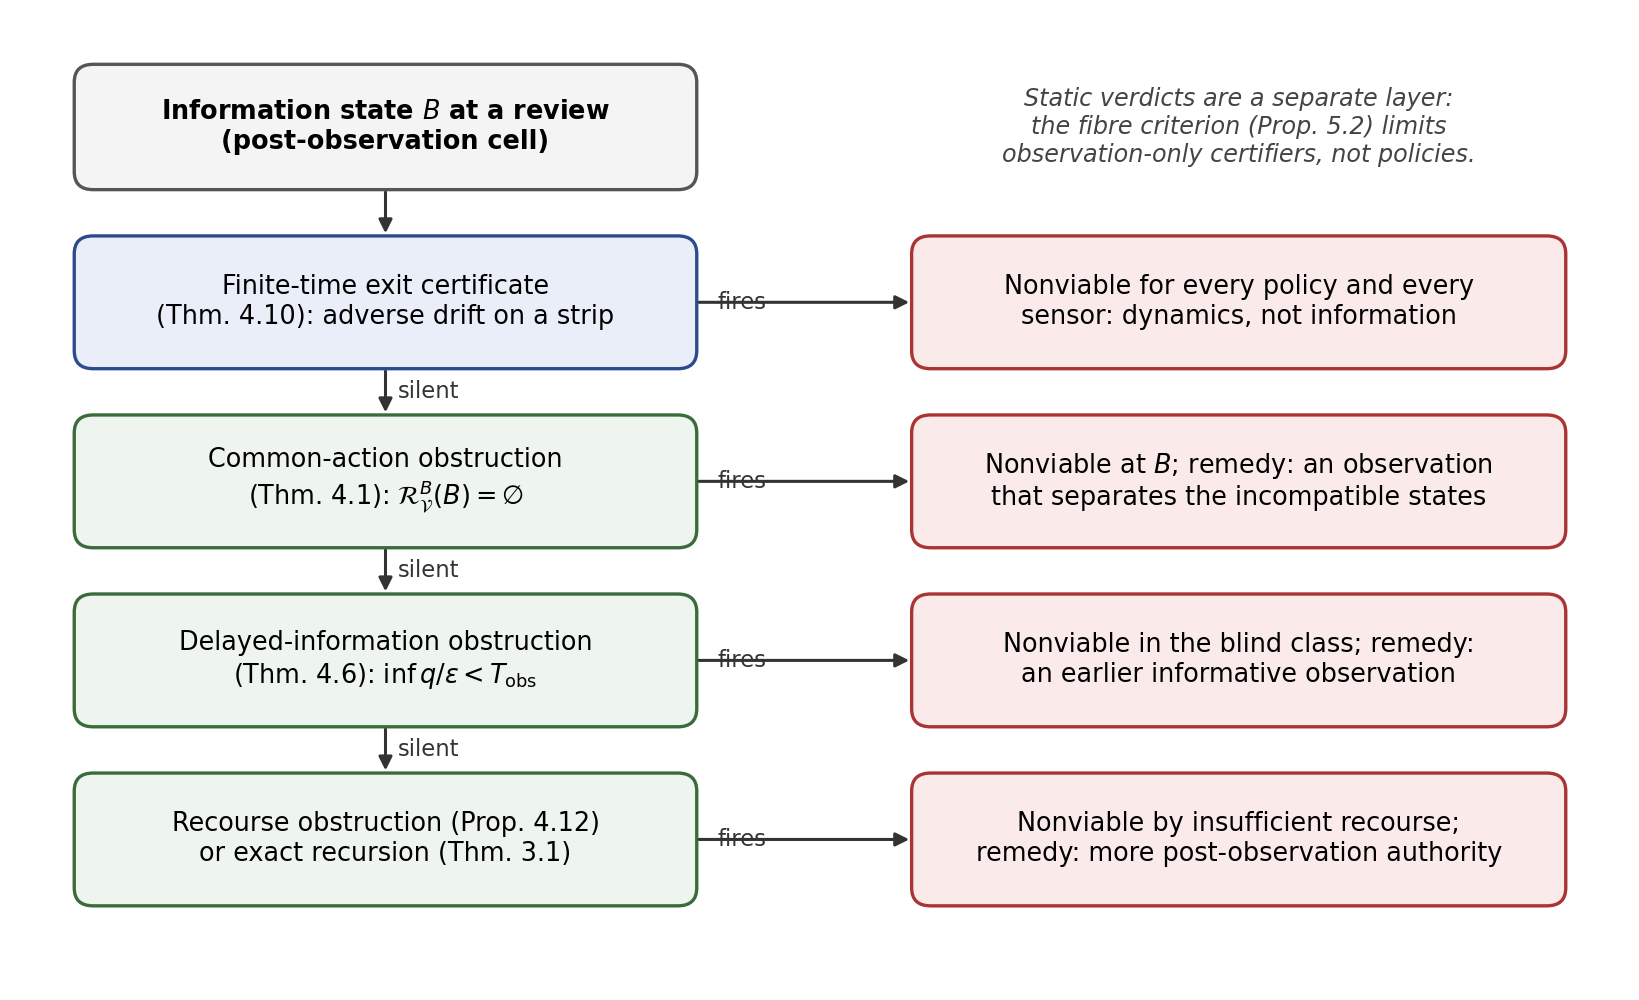
\includegraphics[width=0.9\textwidth]{figs/fig_v73_diagnostic.png}
\caption{The diagnostic use of the calculus at a post-observation information state. Each certificate proves that a specific response correspondence is empty; the mechanism that fires names the design change that could restore the correspondence. The static certification layer (Section~\ref{sec:certification}) constrains verdicts rather than policies and is kept separate.}
\label{fig:diagnostic}
\end{figure}

\subsection{The common-action obstruction}\label{sec:common-action}

The instantaneous obstruction is the static core of the calculus: it certifies nonviability at a single information state without a timing or horizon argument.

\begin{theorem}[common-action obstruction]\label{thm:common-action}
Let $B\subseteq\cV$ be a post-observation information set and consider the held-action review class \hyp{Hold}. Suppose:
\begin{description}[leftmargin=2.6em,itemsep=1pt]
\item[\hyp{C1}] the selected action is held until the next observation;
\item[\hyp{C2}] either $U^B(B)=\varnothing$ (\emph{admissibility obstruction}), or $U^B(B)\ne\varnothing$ and
\begin{equation}\label{eq:common-empty}
\cR^B_\cV(B)=\bigcap_{x\in B}\cR_\cV(x)=\varnothing\qquad\text{(\emph{safety obstruction})};
\end{equation}
\item[\hyp{C3}] (\emph{adverse path, safety case}) for each $a\in U^B(B)$ there exist $x_a\in B\cap\partial\cV$, an active constraint $j_a$, numbers $c_a,\tau_a>0$, and an admissible original-system Carath\'eodory pair $(x_a(\cdot),d_a(\cdot))$ from $x_a$ under the held action $a$, compatible with the pre-review record, with $d_a(t)\in D(x_a(t))$ a.e.\ and $q_{j_a}(x_a(t))\le-c_at<0$ for $0<t<\tau_a$.
\end{description}
Then $B\notin\ERViab_\cI(\cV)$ for the declared class: every compatible state may be individually robustly viable, and the belief is nevertheless nonviable because the state-specific safe actions are incompatible.
\end{theorem}

\begin{proof}
Fix a policy of the class and its held first command $a$. If $a\notin U^B(B)$ it is inadmissible at some compatible state, which is failure by \hyp{Fail}. Otherwise $a\in U^B(B)$, and \eqref{eq:common-empty} says that $a$ fails an active-gradient inequality at some compatible boundary state; \hyp{C3} supplies a realised compatible path from such a state on which the active constraint is strictly negative at arbitrarily small positive times, hence before the next review. The policy was arbitrary within the hold class.
\end{proof}

Hypothesis \hyp{C3} is substantive: a failed gradient test exhibits a disturbance \emph{value} with outward drift, and the certificate needs a disturbance \emph{selection} that realises it along an admissible trajectory. Neither closed graph nor lower semicontinuity of $D$ supplies this (S2.1 gives a closed-graph witness in which a phantom value fails the test while the belief is viable), and a trajectory of the convexified inclusion is not a substitute. The distinction does not make the test less useful---in the polyhedral and finite classes below the path is immediate---but it is what separates a sound certificate from a heuristic.

\paragraph{Farkas form.} When the safe-action constraints over the belief are finitely many affine inequalities $A_iu\le b_i$, stacked as $Au\le b$, the intersection is empty if and only if some $\mu\ge0$ satisfies $\mu^\top A=0$ and $\mu^\top b<0$ \citep{farkas1902,gale1960}: a finite, independently checkable certificate of epistemic infeasibility. Linearity makes the certificate numerically robust---bounded data perturbation degrades the margin $\mu^\top b$ gracefully, and verified approximate multipliers suffice, provided uncertain rows are relaxed toward a \emph{larger} feasible controller set, never a smaller one, since tightening on an unverified worst case can manufacture a false obstruction (S3.1).

\begin{figure}[tb]
\centering
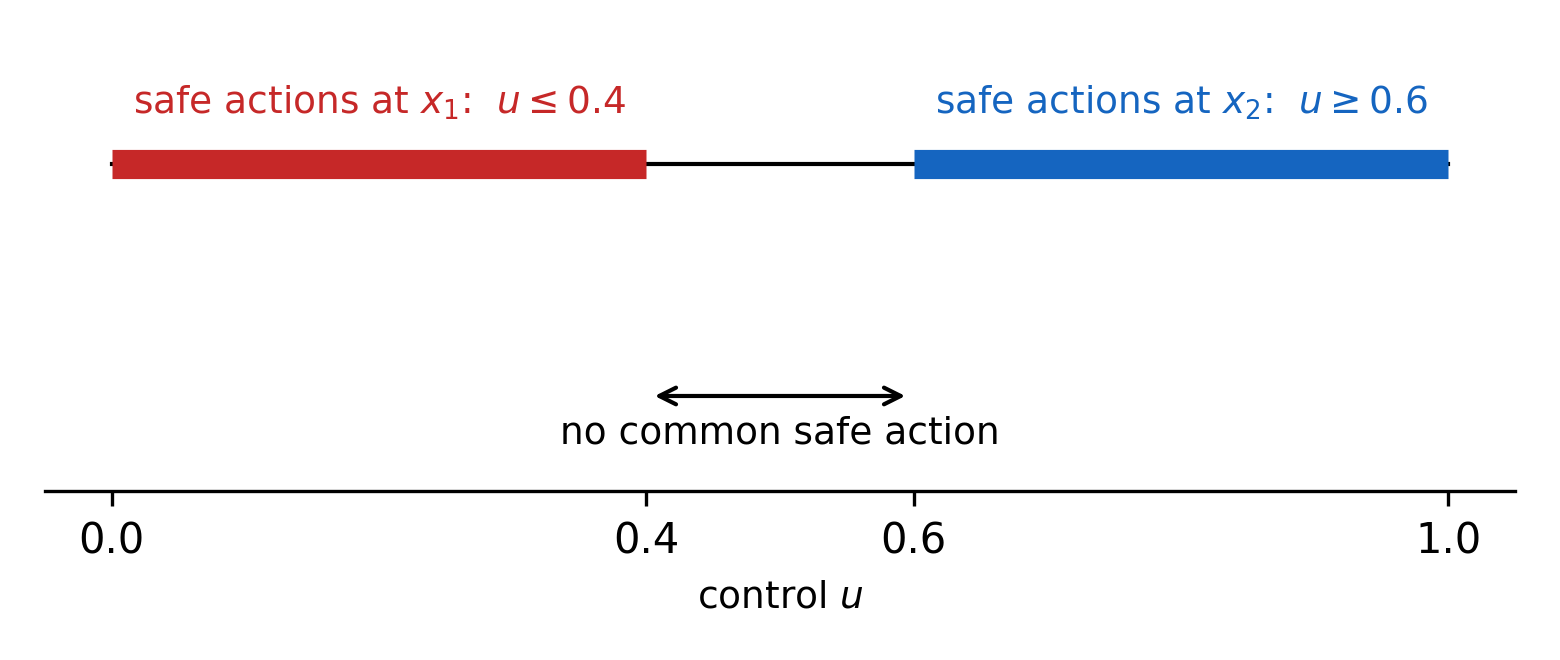
\includegraphics[width=0.6\textwidth]{figs/fig_p2_common_action.png}
\caption{Incompatible safe controls. The states $x_1$ and $x_2$ share an observation but their safe-action sets $[0,0.4]$ and $[0.6,1]$ are disjoint; the Farkas pair $\mu=(\tfrac12,\tfrac12)$ certifies emptiness with margin $0.1$, which shrinks to zero exactly as the two sets come to touch. Any observation separating $x_1$ from $x_2$ restores one-step viability.}
\label{fig:common-action}
\end{figure}

\begin{proposition}[obstruction ladder]\label{prop:ladder}
For the held-action review class, assuming \hyp{C3} at every failed active-gradient test and original-system solutions through the review, the response correspondences are nested,
\[
\Atube(B,\Delta)\;\subseteq\;\cR^B_\cV(B)\;\subseteq\;U^B(B)\qquad(\Delta>0),
\]
and emptiness descends: $U^B(B)=\varnothing\Rightarrow\cR^B_\cV(B)=\varnothing\Rightarrow\Atube(B,\Delta)=\varnothing\Rightarrow B\notin\ERViab_\cI(\cV)$.
\end{proposition}

\begin{proof}
The second inclusion is $\cR_\cV(x)\subseteq U(x)$. For the first, a command in $U^B(B)\setminus\cR^B_\cV(B)$ fails an active-gradient test, and \hyp{C3} supplies an admissible path that exits before every positive review time, so the command is not tube-safe. The last implication is Proposition~\ref{prop:selector}(ii) for policies obliged to hold the first command over this $\Delta$; it says nothing about within-review switching.
\end{proof}

The rungs are strict in general: an instantaneously tangent action may still exit in finite time, which is exactly the gap that \hyp{C3} closes, and the finite recursive correspondence $\cA_N$ joins the ladder only through a sampled-transition model (Figure~S8.1). The dynamic exit certificate of Section~\ref{sec:exit} sits below the ladder: it empties the response set of some compatible state under full information.

\begin{proposition}[sparse common-action witness]\label{prop:helly}
Let $B\subseteq\cV$, let $U\subseteq\R^m$ be compact and convex with $U(x)\subseteq U$ convex and closed, let the dynamics be affine in the control, $f(x,u,d)=f_0(x,d)+f_u(x,d)\,u$, with $D(x)$ compact, and let the $q_j$ be $C^1$. Then each $\cR_\cV(x)$ is a compact convex subset of $U$, and $\bigcap_{x\in B}\cR_\cV(x)=\varnothing$ if and only if it is witnessed by at most $m+1$ compatible states: there are $1\le\ell\le m+1$ states $x_1,\dots,x_\ell\in B$ with $\bigcap_{i\le\ell}\cR_\cV(x_i)=\varnothing$. The admissibility analogue, with $U(x)$ in place of $\cR_\cV(x)$, holds under the same convexity assumptions.
\end{proposition}

\begin{proof}
For fixed $(x,j,d)$ the inequality $\nabla q_j(x)\cdot f(x,u,d)\ge0$ is affine in $u$ and defines a closed half-space, whatever the convexity of $q_j$ in $x$; intersecting over active $j$ and $d\in D(x)$ with the closed convex $U(x)\subseteq U$ gives a compact convex set. If the intersection over $B$ is empty, the finite-intersection property of compact sets yields a finite subfamily with empty intersection, and Helly's theorem in $\R^m$ \citep{helly1923} reduces it to at most $m+1$ members. The converse is immediate.
\end{proof}

\begin{remark}[scope of the count]\label{rem:count}
Convexity is essential: with $U=\R$ and nonconvex safe sets $\{0,1\},\{0,2\},\{1,2\}$ every pair intersects but the triple does not, so no two-state witness exists. The bound also counts \emph{instantaneous} actions, not window-policies. Partition a blind window into $Q$ blocks $I_1,\dots,I_Q$ and let $q+1$ branches be indistinguishable throughout, with scalar input: branch $j\le q$ evolves as $\dot x_j=\mathbf 1_{I_j}(t)(u-1)$ from $x_j(0)=0$ under the floor $x_j\ge0$, forcing $u\equiv1$ on $I_j$, while branch $q+1$ evolves as $\dot x_{q+1}=-u$ from $x_{q+1}(0)=q-\varepsilon$, forcing $\int u\le q-\varepsilon$. The full system is infeasible, yet removing any single branch restores feasibility, so every obstruction involves all $q+1$ branches. For window-policies the governing count is the information--time rank $mQ$, not $m$.
\end{remark}

\begin{proposition}[epistemic emptiness by admissibility: a minimal construction]\label{prop:emptiness}
There is a system with $\Viab(\cV)=\cV\ne\varnothing$ and a non-injective observation $O$ such that every full-fibre initial belief $B_0=O^{-1}(O(S_0))$, $S_0\in\cV$, lies outside $\ERViab_\cI(\cV)$. The mechanism is admissibility: a state-dependent control set leaves a single common action at the merged belief, and that action drifts outward at the boundary.
\end{proposition}

\begin{proof}[Construction]
Take $X=\cV=[1,2]$, $\dot S=u-S$, the unrelaxed nonconvex control sets $U(S)=\{0,S\}$, and the constant observation $O\equiv0$. Under full information $u=S$ gives $\dot S=0$, so every state is viable. Under $O\equiv0$ the only action shared by all $U(S)$ is $0$, so every observation-based policy holds $u=0$ by \hyp{Fail}; then $S(t)=S(0)e^{-t}$ crosses the lower boundary at $t=\log S(0)\le\log2$ and leaves immediately from $S(0)=1$. The construction is Theorem~\ref{thm:common-action}'s safety case at minimal size, with the adverse path explicit; it is epistemic rather than dynamic, since with the constant control set $[0,2]$ in the same plant any $u\equiv m\in(1,2)$ keeps every branch in $[1,2]$. Convexifying the controller sets to $[0,S]$ is a different problem in which $u\equiv1$ is common and safe; no such convexification is used.
\end{proof}

\subsection{The delayed-information obstruction}\label{sec:delayed}

Information may be accurate yet arrive too late. The second certificate turns the timing of the first informative observation into an explicit bound.

\begin{theorem}[delayed-information obstruction]\label{thm:delayed}
Let $B_0\subseteq\cV$ be a compact initial post-observation cell and $\Tobs>0$ a blind horizon. Fix a policy class $\Pi$ of \emph{blind-window controls}: by default all implementable measurable controls on $[0,\Tobs)$, or a declared subclass such as the whole-window hold class. Suppose:
\begin{description}[leftmargin=2.6em,itemsep=1pt]
\item[\hyp{D1}] for each control history in $\Pi$, every compatible realisation produces the same observation record on $[0,\Tobs)$ while safe, so no branch-dependent observation can change the control before exit;
\item[\hyp{D2}] there are a $C^1$ function $q$ on a neighbourhood of the relevant trajectories with $\cV\subseteq\{q\ge0\}$, a number $\varepsilon>0$ and a strip level $a>\max_{B_0}q$ such that, \emph{for every} $u(\cdot)\in\Pi$, there exist a minimiser $x_u\in B_0$ of $q$ and an admissible realisation $d_u(\cdot)$ with an absolutely continuous original-system solution from $x_u$ that follows the common record of \hyp{D1} until exit, exists through any first contact with $q=0$ until it reaches $q<0$ or $\Tobs$, and satisfies, for a.e.\ pre-exit time in the closed strip $0\le q(x(t))\le a$ (boundary contact included),
\begin{equation}\label{eq:drift}
\frac{d}{dt}q(x(t))=\nabla q(x(t))\cdot f(x(t),u(t),d_u(t))\le-\varepsilon;
\end{equation}
\item[\hyp{D3}] the timing bound
\begin{equation}\label{eq:timing}
\Tobs>\frac{\inf_{x\in B_0}q(x)}{\varepsilon}.
\end{equation}
\end{description}
Then no policy of $\Pi$ is viable from $B_0$. For the unrestricted observation-based class this says $B_0\notin\ERViab_\cI(\cV)$; for a proper declared subclass it asserts class-relative nonviability only.
\end{theorem}

\begin{proof}
Fix a policy of $\Pi$. By \hyp{D1} it reduces on $[0,\Tobs)$ to one blind control $u$ (an action inadmissible on a compatible branch already fails). Take the minimiser and realisation of \hyp{D2}, put $h(t)=q(x(t))$, $m=h(0)=\min_{B_0}q\ge0$ and $t_*=m/\varepsilon<\Tobs$, and suppose there is no strict violation by some $t_1\in(t_*,\Tobs)$. As long as $0\le h\le a$, \eqref{eq:drift} integrates to $h(t)\le m-\varepsilon t$; the path cannot first leave the strip through $h=a$, since its derivative is strictly negative there, and at a contact $h=0$ it cannot remain nonnegative, for the same reason. Hence $0\le h(t_1)\le m-\varepsilon t_1<0$, a contradiction. The case $m=0$ is included: negative drift is required \emph{at} the boundary, so contact alone is never mistaken for exit. The quantifier is $\forall\pi\,\exists(x_u,d_u)$; the theorem does not demand that every branch drift downward and need not detect a failure caused only by a non-minimiser branch.
\end{proof}

Condition \eqref{eq:drift} is a condition on the data, not on the policies, and \eqref{eq:timing} is a sufficient timing condition: evading it does not establish viability. Inverted, the bound is a design requirement---the first informative observation must precede the enforced exit time $\inf q/\varepsilon$ (Figure~\ref{fig:timing}). The common-action obstruction is a formal zero-margin counterpart of this certificate, but the two remain distinct: one is a local action-feasibility condition, the other a finite-time survival condition, and they are not related as a $\Tobs\to\infty$ limit (S2.5).

\begin{figure}[tb]
\centering
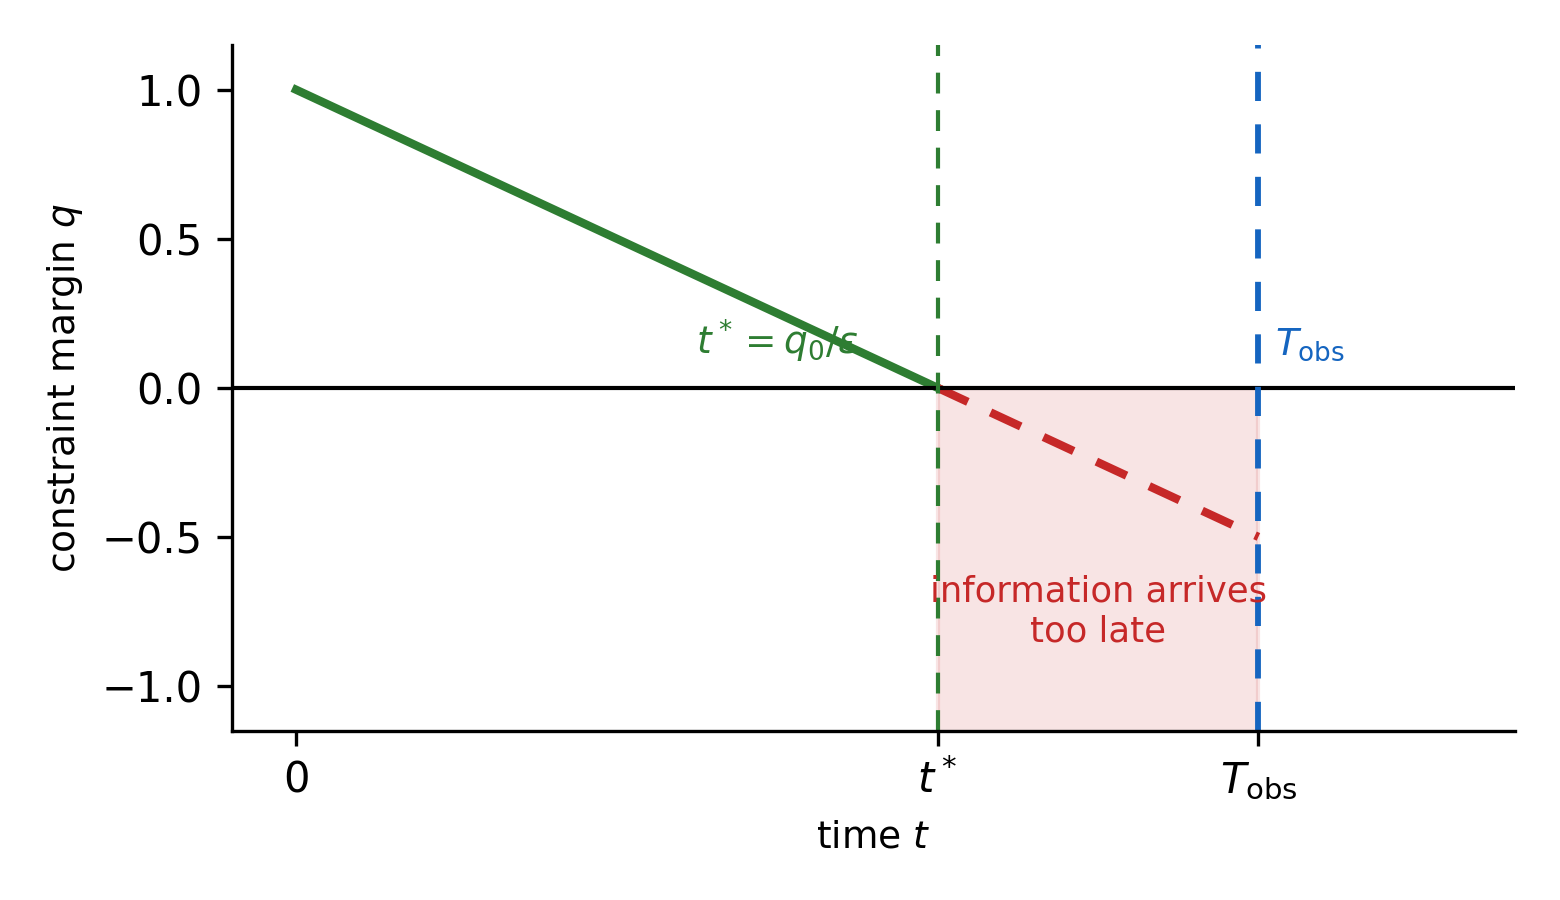
\includegraphics[width=0.58\textwidth]{figs/fig_p2_timing.png}
\caption{Delayed information. Under the compatible adverse-path hypothesis a still-safe branch reaches $q=0$ by $t^*=q_0/\varepsilon<\Tobs$, and continuing the adverse path while it remains safe forces strict exit before the first informative observation (Theorem~\ref{thm:delayed}). The bound need not equal the first contact time.}
\label{fig:timing}
\end{figure}

\begin{remark}[threshold form]\label{rem:sigma}
For a declared blind-window class $\Pi$ let the \emph{guaranteed survival time} be
\[
\sigma^*_\Pi(B_0)=\sup_{u(\cdot)\in\Pi}\ \inf_{x_0\in B_0,\ d(\cdot)}\tau(x_0,u,d),
\]
the infimum over branches that remain observation-equivalent on $[0,\Tobs)$ and $\tau$ the first violation time. Then $\sigma^*_\Pi(B_0)<\Tobs$ implies that no policy of $\Pi$ is viable from $B_0$, because before $\Tobs$ no policy can condition its action on which branch realises. Under \hyp{D1}--\hyp{D2}, for every control in $\Pi$ some branch exits by $\inf q/\varepsilon$, so $\sigma^*_\Pi(B_0)\le\inf q/\varepsilon$ and \eqref{eq:timing} certifies the threshold; the threshold may be strictly smaller, in which case nonviability holds even when \eqref{eq:timing} fails. Emptiness of this blind-window response correspondence is the timing analogue of the tube and common-action rungs.
\end{remark}

For finite blind-window classes (finite $B_0$, hold-until-$\Tobs$ controls from a finite set, or piecewise-constant controls on a finite partition) the drift hypothesis is checked by enumeration of controls together with, for each, an admissible adverse solution with the closed-strip property; enumeration alone does not supply the continuous realisation. Over polytope-declared classes the check is exact and finite.

\begin{theorem}[linear-programming instantiation]\label{thm:lp}
Let the blind window have $K$ discrete steps and finitely many branches $j\in J$ with robust affine dynamics $x^+=A_jx+B_ju+E_jw$, $w\in W_j$ a polytope, known initial branch states $x_{j,0}$, polyhedral safe set $\cV=\{x:Fx\le g\}$, and declared blind-window class $\Pi_B=\{(u_0,\dots,u_{K-1}):u_k\in U\}$ for a polytope $U$. Then:
\begin{enumerate}[label=(\roman*),leftmargin=2.2em,itemsep=1pt]
\item $\sigma^*(B_0;\Pi_B)$ is computed exactly by at most $\lceil\log_2K\rceil+1$ linear programmes of size polynomial in $K$, $|J|$ and the description lengths of $U$, $W_j$, $\cV$; with rational data every step is exact;
\item when the per-step disturbance choices are independent, infeasibility at horizon $K$ is certified by Farkas multipliers---nonnegative weights on the (branch, step, floor) rows whose aggregate control projection vanishes and whose aggregate constant is negative---the timing certificate in adjoint-row form;
\item the programme's feasible set is the declared class itself, so the computation is sound and complete over $\Pi_B$: no relaxation gap arises;
\item the declaration is load-bearing: the per-step polytope programme may be a strict outer relaxation of a separately declared whole-window hold class $\Pi_{\mathrm{hold}}=\{(u,\dots,u):u\in\{-1,+1\}\}$, with a survival gap that grows without bound in $K$.
\end{enumerate}
\end{theorem}

\begin{proof}
Unrolling, $x_{j,k}=A_j^kx_{j,0}+\sum_{i<k}A_j^{k-1-i}(B_ju_i+E_jw_{j,i})$, so for branch $j$, step $k$ and floor row $r$ the robust inequality $F_rx_{j,k}\le g_r$ for all independently selectable $w_{j,i}\in W_j$ is the single linear row
\begin{equation}\label{eq:lprow}
\sum_{i=0}^{k-1}F_rA_j^{k-1-i}B_ju_i\;\le\;g_r-F_rA_j^kx_{j,0}-\sum_{i=0}^{k-1}h_{W_j}\!\bigl(E_j^\top(A_j^{k-1-i})^\top F_r^\top\bigr),
\end{equation}
each support value being a linear programme over $W_j$, precomputed once (for coupled disturbance paths the joint support replaces the sum). The horizon-$K'$ feasibility programme $\{Gu\le b\}$ in $(u_0,\dots,u_{K'-1})$ has one row per (branch, step, floor) plus the rows of $U$; its rows for a shorter horizon are a subset of those for a longer one, so feasibility is monotone and $\sigma^*=\max\{K'\le K:\text{feasible}\}$ is found by bisection, giving (i). Farkas' lemma gives (ii), indexing the multipliers by (branch, step, floor). Claim (iii) is definitional. For (iv) take the non-decaying branches $z^+=z\pm u$ with floor $z\ge1$ from $z_0=2$: either hold survives exactly one blind step, whereas the relaxation $U=[-1,1]$ admits $u\equiv0$, which survives every horizon (S2.6).
\end{proof}

\begin{example}[decaying threshold, and the hold-class gap]\label{ex:relax-gap}
Two branches share $z^+=\tfrac9{10}z\pm u$ from a common $z_0$, floor $z\ge1$, declared class $u_k\in[-1,1]$. The branch sum $z^+_k+z^-_k=2(\tfrac9{10})^kz_0$ is control-invariant, so both floors force $z_0\ge(\tfrac{10}9)^k$ at every step: the window-$K$ programme is feasible exactly when $z_0\ge(\tfrac{10}9)^K$. The level-$k$ Farkas certificate is the pair of floor rows summed---their control coefficients cancel pairwise, the discrete image of pooled adjoint rows---and $u\equiv0$ attains feasibility on the boundary, so the programme is a complete characterisation of this class. The unbounded gap of Theorem~\ref{thm:lp}(iv) concerns a \emph{different}, non-decaying system and a whole-window hold class, and it is specifically a gap between that hold class and its per-step polytope relaxation: in the per-step finite class $\{-1,+1\}^K$ the alternating sequence $+1,-1,+1,\dots$ keeps both branches of $z^+=z\pm u$ safe from any $z_0\ge2$ (verification record, S7).
\end{example}

\subsection{The finite-time exit certificate}\label{sec:exit}

The base obstruction operates before any observation argument: it certifies membership in the full-information ``shadow'' of the kernel \citep{aubin2001,aubin2002}, and when it fires no monitoring design can rescue viability.

\begin{theorem}[finite-time exit certificate]\label{thm:exit}
Let $q:X\to\R$ be $C^1$ with $\cV\subseteq\{q\ge0\}$ and suppose:
\begin{description}[leftmargin=2.6em,itemsep=1pt]
\item[\hyp{E1}] there are $a>0$ and $\varepsilon>0$ such that on the strip $\cS_a=\{x:0\le q(x)\le a\}$
\begin{equation}\label{eq:isaacs}
\sup_{u\in U(x)}\ \inf_{d\in D(x)}D^+q\bigl(x;f(x,u,d)\bigr)\le-\varepsilon\qquad\forall x\in\cS_a;
\end{equation}
\item[\hyp{E2}] (\emph{adverse realisation for the declared control class}) for every admissible control history of the class and every $x_0\in\cS_a$ there is a compatible absolutely continuous original-system trajectory with a measurable disturbance $d(t)\in D(x(t))$, defined beyond $q(x_0)/\varepsilon$ unless it has already reached $q<0$, satisfying $\frac{d}{dt}q(x(t))\le-\varepsilon$ a.e.\ while $0\le q(x(t))\le a$ before exit, and continuing through first contact long enough to decide strict exit.
\end{description}
Then for every control of the declared class and every $x_0\in\cS_a$ an admissible trajectory strictly violates $q\ge0$ before every time strictly greater than $q(x_0)/\varepsilon$; the infimum of strict-violation times is at most $q(x_0)/\varepsilon\le a/\varepsilon$, and viability fails in the class.
\end{theorem}

\begin{proof}
Fix a control and the pair of \hyp{E2}; put $h(t)=q(x(t))$ and $t_0=h(0)/\varepsilon$. If the pair stayed in $\{q\ge0\}$ through some $t_1>t_0$ before its guaranteed continuation ends, it could not first cross upward through $h=a$, and integrating the drift on the still-safe portion gives $0\le h(t_1)\le h(0)-\varepsilon t_1<0$, a contradiction. The drift is never integrated on a path after it has left the strip.
\end{proof}

Condition \eqref{eq:isaacs} has the control-before-disturbance (Isaacs) reading and is information-independent; \hyp{E2} is what makes the pointwise condition a pathwise certificate, and it is a hypothesis about the original game that the standing solution-existence conditions do not discharge (they give a solution for each fixed selection pair, not a drift-consistent adversarial selection coupled to a policy). For an open-loop control one admissible path may depend on the control; disturbance-reactive closed-loop classes need their own compatible-solution premise, for which a state-uniform $d^*$ with $\sup_{u\in U(x)}\nabla q(x)\cdot f(x,u,d^*)\le-\varepsilon$ on the strip is one sufficient condition. A state-dependent barrier may be used with output feedback; only an observation-only barrier subclass must be fibre-constant.

\begin{remark}[comparison-function form]\label{rem:comparison}
If $\dot q\le-\alpha(q)$ with $\alpha:(0,a]\to(0,\infty)$ holds along a compatible adverse trajectory while $q>0$ and $\int_0^{q(x_0)}\dd s/\alpha(s)<\infty$, comparison bounds the time of \emph{first boundary contact}; it does not alone give strict exit from the closed set---the solution of $\dot q=-\sqrt q$ from $q(0)=1$ reaches zero at time two and may stay there. Strict exit requires negative drift at or through contact, as in \hyp{E2}.
\end{remark}

\subsection{The post-observation recourse obstruction}\label{sec:recourse}

The certificates so far fire before information discriminates. The complementary mode---\emph{insufficient post-observation recourse}---is one in which a common blind-window control keeps every branch safe, yet no observation-adapted control can recover every branch once the distinguishing observation arrives. The finite recursion captures it exactly (a four-state instance in which every one-step certificate is silent is S6.3); the following certificate detects it in continuous time for affine systems. It relaxes the post-observation class upward---an oracle grants each stored branch its own controller whether or not the sensor reveals that much---so it is sound but not complete.

\begin{proposition}[oracle-recourse obstruction]\label{prop:recourse}
For each branch $\theta$ and fixed exogenous disturbance scenario $d(\cdot)$ let the dynamics be affine in state and input, $\dot x_\theta=A^d_\theta(t)x_\theta+g^d_\theta(t)+B^d_\theta(t)u$, with bounded measurable coefficients on $[0,T]$ that do not depend on the controlled trajectory; scenarios are exogenous (each admissible $d(\cdot)$ remains admissible under every policy). Let the safety facets be affine, $q_j(x)=c_j^\top x+b_j$ with safety $q_j\ge0$, let $U\subseteq\R^m$ be compact convex, and let branches $x_1,\dots,x_L\in B_0$ be observation-equivalent on $[0,\tau)$ with horizon $T>\tau$. For a label $\ell=(\theta,j,t)$, $t\in(\tau,T]$, let $\bar x^d_\theta$ be the zero-control trajectory, $X^d_\theta(t,\sigma)$ the transition matrix, $\beta^d_\ell=q_j(\bar x^d_\theta(t))$ the zero-control facet margin, and
\[
k^d_\ell(\sigma)=\mathbf 1_{\{\sigma\le t\}}\bigl(B^d_{\theta}(\sigma)\bigr)^\top\bigl(X^d_\theta(t,\sigma)\bigr)^\top\nabla q_j
\]
the input kernel. For weights $\lambda_\ell\ge0$, $\sum_\ell\lambda_\ell=1$, define
\begin{equation}\label{eq:gamma}
\Gamma_h(\lambda)=\inf_{d(\cdot)}\Bigl\{\sum_\ell\lambda_\ell\beta^d_\ell+\int_0^\tau h_U\Bigl(\sum_\ell\lambda_\ell k^d_\ell(\sigma)\Bigr)\dd\sigma+\sum_\ell\int_\tau^Th_U\bigl(\lambda_\ell k^d_\ell(\sigma)\bigr)\dd\sigma\Bigr\}.
\end{equation}
If $\Gamma_h(\lambda)<0$ then $B_0\notin\ERViab_\cI(\cV)$: for every measurable information-adapted policy, at least one stored branch violates a facet under the chosen exogenous scenario (the branch may depend on the policy).
\end{proposition}

\begin{proof}
If the infimum is negative, some exogenous scenario $d^*$ has a negative bracket, and it remains admissible against every policy. For that scenario, variation of constants and affinity of the facets give the \emph{exact} identity $q_j(x^{u,d^*}_\theta(t))=\beta^{d^*}_\ell+\int_0^\tau(k^{d^*}_\ell)^\top w+\int_\tau^t(k^{d^*}_\ell)^\top u_\theta$, where $w$ is the one common window signal (the blind-window reduction of Theorem~\ref{thm:delayed}) and $u_\theta$ the branch's post-reveal signal. Each pairing is bounded above by its support value, so the $\lambda$-weighted facet sum is at most the bracket, hence strictly negative; a strictly negative weighted sum forces some facet strictly negative along its branch. The window signal was arbitrary, so every policy of the class fails (S2.7, including the attainment-special $\phi_U$ variant).
\end{proof}

The state-independent input coefficient and affine facets are load-bearing: for state-dependent $B(x)$ or nonlinear facets the identity is only first-order, and the certificate may fire falsely unless a validated one-sided remainder is added (S2.7 records an explicit scalar counterexample to the control-affine generalisation). Variation of constants evaluates the bracket for a fixed scenario; an admissible scenario with a negative bracket is already a failure witness, whereas a negative lower bound on the infimum is not.

\begin{example}[three branches, delayed recourse]\label{ex:three-branch}
Branches $j=1,2,3$ run the planar double integrator $\dot p=v$, $\dot v=u$ without disturbance from $p_j(0)=\tfrac{34}{25}n_j$, $v_j(0)=n_j$, where $n_1=(1,0)$, $n_2=(-\tfrac35,\tfrac45)$, $n_3=(-\tfrac35,-\tfrac45)$; the actuator set is the hexagon $U=\co\{\pm n_1,\pm n_2,\pm n_3\}$; safety is $n_i^\top p\le2$ for $i=1,2,3$ with $\|v\|_\infty\le\tfrac65$; the realised branch is revealed at time $\tau$. Every branch is viable under full information (brake along $-n_j$ for one second; peak critical position $\tfrac{34}{25}+\tfrac12=\tfrac{93}{50}<2$), and $u\equiv0$ keeps every branch strictly safe through any blind window of length below $\tfrac{16}{25}$, so no instantaneous or blind-window certificate fires. The labels $(j,\,n_j^\top p\le2,\,\tau+1)$ have zero-control margins $\beta_j=\tfrac{16}{25}-\tau-1$ and kernels $\mathbf 1_{\{\sigma\le\tau+1\}}(\tau+1-\sigma)n_j$; the weights $\lambda=(\tfrac38,\tfrac5{16},\tfrac5{16})$ pool the pre-observation kernel to zero, and
\[
\Gamma_h(\tau)=\Bigl(\tfrac{16}{25}-\tau-1\Bigr)+\sum_j\lambda_j\int_\tau^{\tau+1}(\tau+1-\sigma)\dd\sigma=\tfrac7{50}-\tau.
\]
For $\tau>\tfrac7{50}$ the certificate fires and the triple is nonviable---the blind window accumulates braking liability that the post-observation authority cannot discharge on every branch at once---while hold-then-brake is safe exactly to $\tau=\tfrac7{50}$: the threshold is exact. The obstruction is genuinely three-way: at $\tau=\tfrac15$ every pair of branches is jointly viable under a common blind control (worst critical positions $\tfrac{2469}{1250}$ and $\tfrac{2419}{1250}$, Figure~\ref{fig:recourse}), so six of the seven nonempty priors over these branches are viable at a delay where the triple is not; $\Gamma_h(\tfrac15)=-\tfrac3{50}$. All quantities are exact rationals (S3.4, S7).
\end{example}

\begin{figure}[tb]
\centering
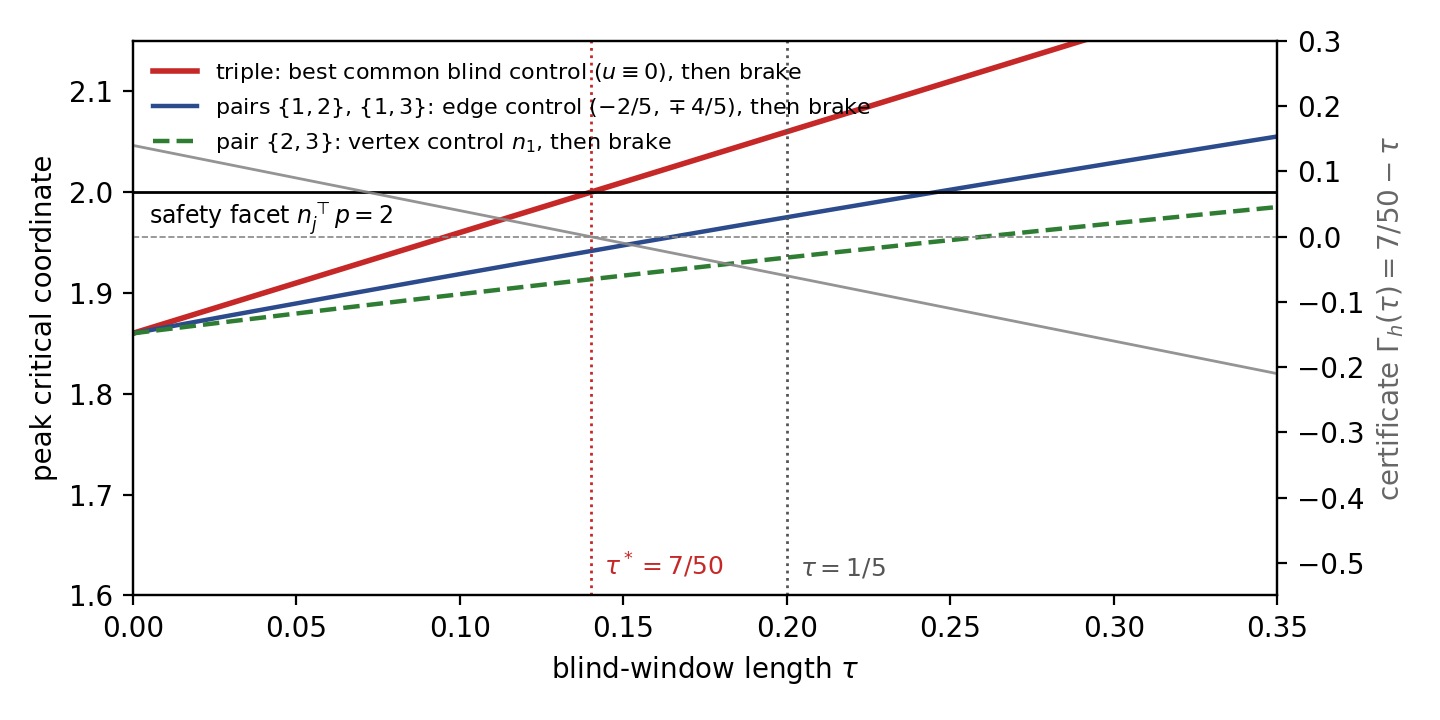
\includegraphics[width=0.8\textwidth]{figs/fig_v73_recourse.png}
\caption{The three-branch recourse instance of Example~\ref{ex:three-branch}. Peak critical coordinate after optimal braking as a function of the blind-window length $\tau$, for the triple under its best common blind control and for the pairs under the stated pair controls; the facet is $2$. The triple fails for $\tau>7/50$, exactly where the certificate $\Gamma_h(\tau)=7/50-\tau$ (grey, right axis) becomes negative, while every pair is still viable at $\tau=1/5$.}
\label{fig:recourse}
\end{figure}
